\section{Champ magnétique de la bobine fixe}
\label{mesures champ}
Lorsque nous avons dimensionné notre bobine fixe (voir le chapitre \textbf{REFERENCE} p. \textbf{REFERENCE}, nous avions estimé que le champ nécessaire pour le bon fonctionnement de notre haut-parleur était de $0.1$\tesla.  Afin d'engendrer un tel champ avec un courant de $1$\ampere \, et un entrefer de $0.5$\centi\meter \,de longueur, nous avions conclu que la bobine devait avoir $400$ tours. Cependant, lors de notre raisonnement, nous avions négligé la "perte" de champ en dehors de l'entrefer. Afin de compenser cette perte et donc d'obtenir notre champ de $0.1$\tesla, nous avons exagéré le nombre de tours de la bobine lors de sa confection matérielle ($\cong 550$ tours). 
Durant une séance de laboratoire, nous avons mesuré au moyen d'un teslamètre, le champ dans l'entrefer de la bobine. Celui-ci s'élève à $112$\milli \tesla \, pour un courant de $0.98$ \ampere \,circulant dans le solénoïde et une tension de $9.1$ \volt. Nos prévisions se sont donc avérées relativement bonnes.

\begin{figure}[h!]
\begin{center}
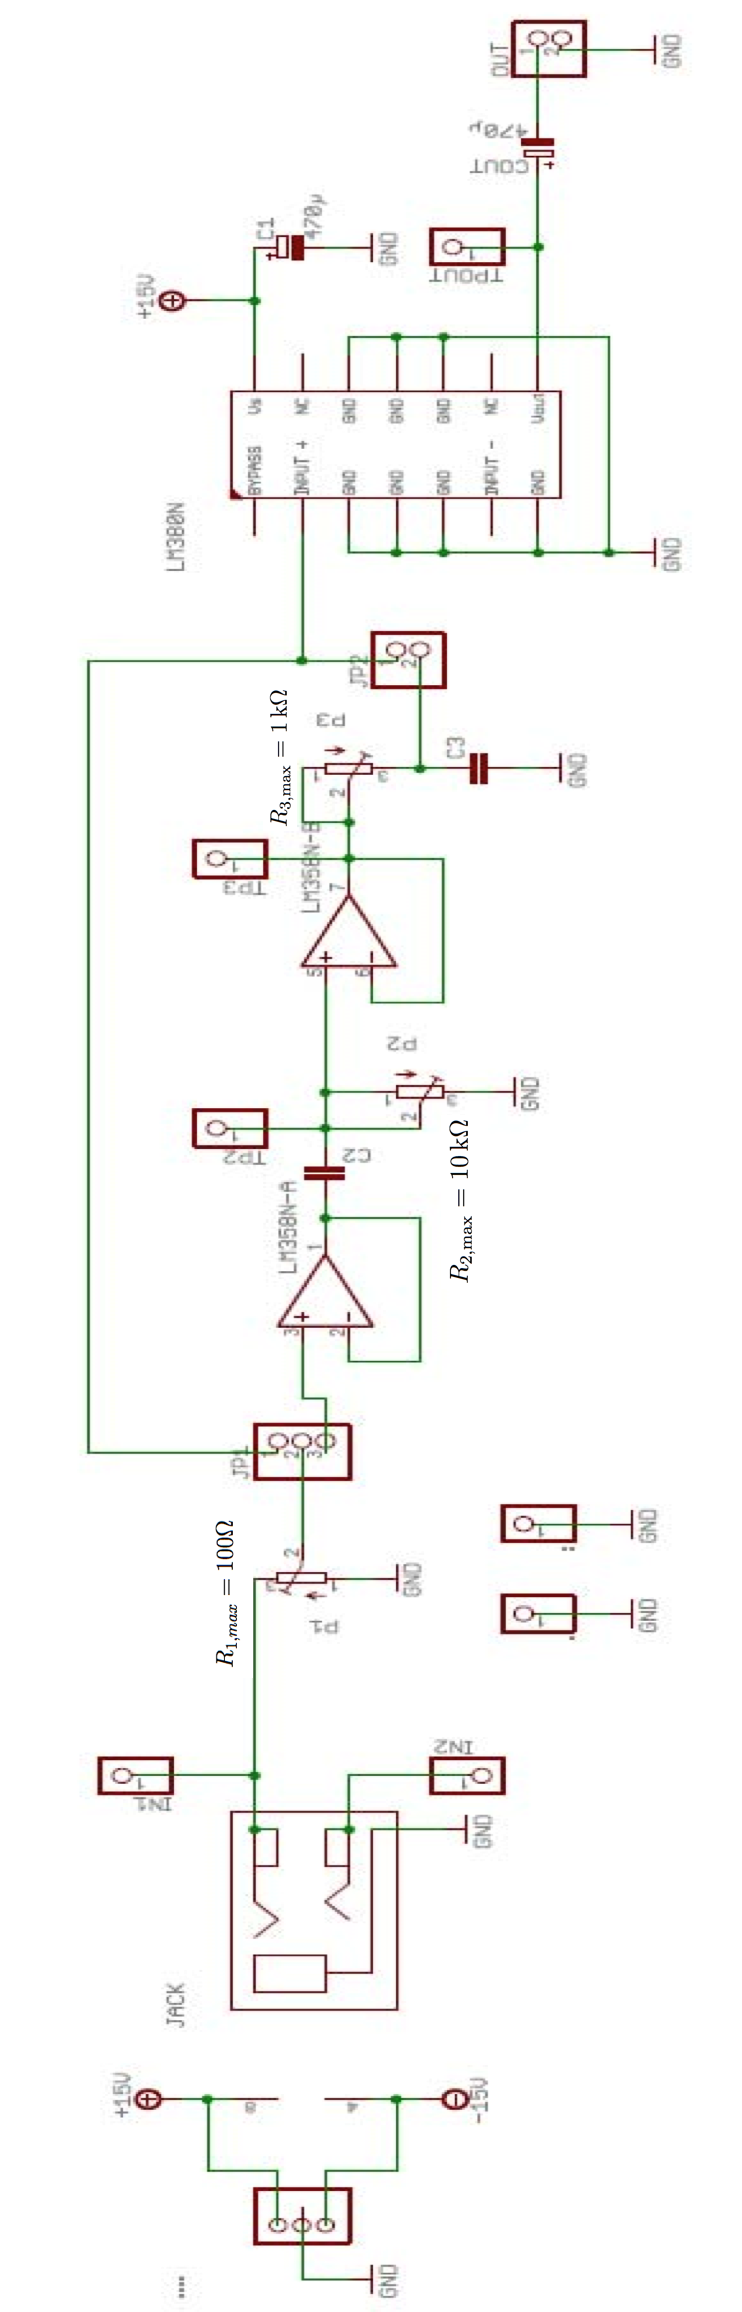
\includegraphics[width=\textwidth]{img/circuitcomplet} 
\end{center}
\caption{Schema complet du circuit imprimé}		
\label{circuitcomplet}		
\end{figure}